\begin{enumerate}
	\item The idea to check for intimate pairs is to create a Voronoi diagram, then create a Delaunay diagram. If we have an edge of the Delaunay diagram, linking two points $p_i$ and $p_j$, and this edge intersects with the edge of the Voronoi diagram separating those two points, then $p_i$ and $p_j$ are intimate.\\
To prove it first it's obvious that for a given point, the only possible intimate points are the direct neighbors of it in the Voronoi diagram. The other points being further away, at least one of the direct neighbor would be inside the circle described in the definition of intimate points.\\
Then why do we need the edge in the Delaunay diagram intersecting the edge in the Voronoi diagram? Well if we have only two points ($p_1$ and $p_2$) in the Voronoi diagram, then obviously the edge linking the two points (in the Delaunay diagram) intersects the edge separating those points in the Voronoi diagram. Now as we can see on Figure \ref{fig:q11}, if we add a point $p_3$ in the \textit{intimate circle} then the edge separating $p_1$ and $p_2$ is going to be shorten where it intersects with the edge separating $p_1$ and $p_3$ and the edge separating $p_2$ and $p_3$. After this change in the Voronoi diagram the edge linking $p_1$ and $p_2$ will not intersect with the edge in the Voronoi diagram anymore. Yet if $p_3$ is added outside this \textit{intimate circle} then the edge separating $p_1$ and $p_2$ is gonna be shorten but less and would still intersect the Delaunay diagram.
\begin{figure}[ht]
  \centering
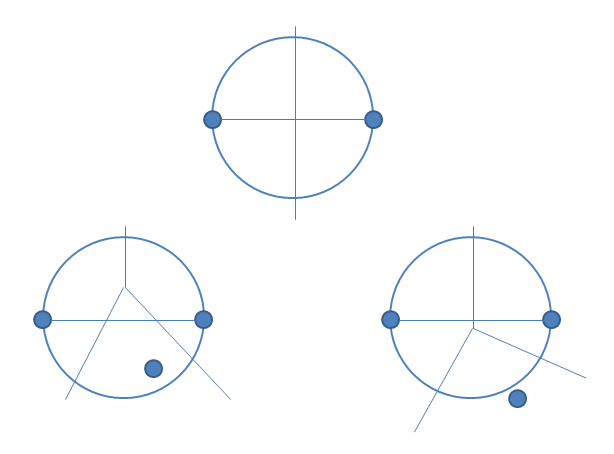
\includegraphics[width=0.7\textwidth]{q11}%
\caption{Illustration of the proof}%
\label{fig:q11}%
\end{figure}
\clearpage
For the running time, as we've seen in class, the Voronoi diagram can be build in O($n\log n$). The Delaunay diagram can be created in O($n$) since we have the Voronoi diagram we just need to link every vertex with their neighbors. After creating the Voronoi diagram we can have a data structure where we have the neighbors of each point and their separating edge and can access them in O(1). And then while we run the algorithm for the Delaunay diagram, every time we add an edge for the diagram we can check if it intersect the edge in the Voronoi diagram and if it does we can keep those points in a data structure. Those calcalations are done in O(1) so it doesn't add complexity in the algorithm. Finally the running time is then: O($n\log n$)+O($n$) $\leq$ O($n \log n$).\\
(source for Delaunay diagram: http://en.wikipedia.org/wiki/Delaunay\_triangulation)
\item We can prove it by contradiction, so let's say there exists a minimum spanning tree where at least one edge is linking two non-intimate points ($p_i$ and $p_j$). So this means there's a point $p_k$ closer to $p_j$ and to $p_i$. This $p_k$ is either not connected to neither of those two points or it's connected to only one of them. $p_k$ cannot be connected to both of them otherwise we have a loop.\\
Now if it's connected to one of them, the subtree with vertices $\{$$p_i$,$p_j$,$p_k$$\}$ should be a minimum spanning tree too. But it is not because the only minimum spanning tree is the one with path $p_i$-$p_k$-$p_j$, yet $p_k$ cannot be connected to both points.\\
If $p_k$ is not connected to either $p_i$ or $p_j$, this means there is a subtree with $p_k$ and this subtree is connected to the subtree $p_i$-$p_j$ with an edge from a vertex $p_x$ to either $p_i$ or $p_j$ and $p_x \neq p_k$. Let's say $p_x$ is connected to $p_i$ it's not a minimum spanning tree because if we remove the edge between $p_i$ and $p_j$ and add an edge $p_k$-$p_j$ we have a smaller spanning tree. Respectively if $p_x$ is connected to $p_j$ and we remove the edge between $p_i$ and $p_j$ and add an edge $p_k$-$p_i$ we have a smaller spanning tree (for a better understanding, see Figure \ref{fig:q12}. So we cannot end with a minimum spanning tree if $p_i$ and $p_j$ are directly connected and not intimate.
\begin{figure}[ht]
  \centering
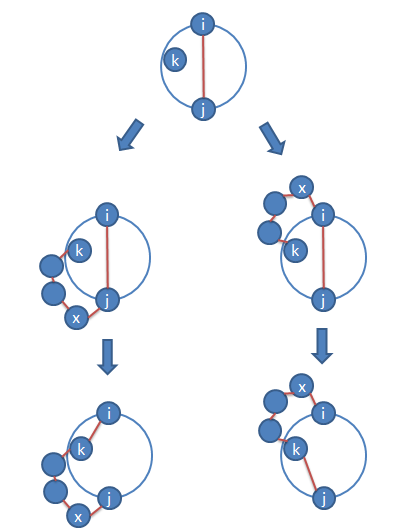
\includegraphics[width=0.5\textwidth]{q12}%
\caption{Illustration of the proof}%
\label{fig:q12}%
\end{figure}
\clearpage
\end{enumerate}